\documentclass[11pt]{article}
\usepackage{amssymb}
\usepackage{amsthm}
\usepackage{enumitem}
\usepackage{physics,amsmath}
\usepackage{bm}
\usepackage{adjustbox}
\usepackage{mathrsfs}
\usepackage{graphicx}
\usepackage{siunitx}
\usepackage[mathscr]{euscript}

\title{\textbf{Solved selected problems of Classical Mechanics - Gregory}}
\author{Franco Zacco}
\date{}

\addtolength{\topmargin}{-3cm}
\addtolength{\textheight}{3cm}

\newcommand{\hatr}{\bm{\hat{r}}}
\newcommand{\hatx}{\bm{\hat{x}}}
\newcommand{\haty}{\bm{\hat{y}}}
\newcommand{\hatz}{\bm{\hat{z}}}
\newcommand{\hatth}{\bm{\hat{\theta}}}
\newcommand{\hatphi}{\bm{\hat{\phi}}}
\newcommand{\hatrho}{\bm{\hat{\rho}}}
\newcommand{\ngrad}[1]{\text{grad}_{\bm{#1}}}

\theoremstyle{definition}
\newtheorem*{solution*}{Solution}
\renewcommand*{\proofname}{\bf{Solution}}

\begin{document}
\maketitle
\thispagestyle{empty}

\section*{Chapter 14 - Hamilton's equations and phase space}

\begin{proof}{\textbf{14.1}}
    We want to find the Legendre transform $G(v_1, v_2, w)$ of the function
    $$F(u_1, u_2, w) = 2u_1^2 - 3u_1u_2 + u_2^2 + 3wu_1$$
    where $w$ is a passive variable.
    Then we have that
    \begin{align*}
        v_1 &= \frac{\partial F}{\partial u_1} = 4u_1 -3u_2 + 3w\\
        v_2 &= \frac{\partial F}{\partial u_2} = -3u_1 + 2u_2
    \end{align*}
    So by replacing $u_2 = v_2/2 + 3u_1/2$  in the formula for $v_1$ we get
    that the inverse formula for $u_1$ is
    \begin{align*}
        u_1 &= -2v_1 - 3v_2 + 6w
    \end{align*}
    Plugging this value in the formula for $u_2$ gives us
    \begin{align*}
        u_2 &= -3v_1 - 4v_2 + 9w
    \end{align*}
    Using the Legendre transform equation we have that
    \begin{align*}
        G(v_1, v_2, w) &= u_1v_1 + u_2v_2 - F(u_1, u_2, w)\\
        &= (-2v_1 - 3v_2 + 6w)v_1 + (-3v_1 - 4v_2 + 9w)v_2\\
        &\quad - (2(-2v_1 - 3v_2 + 6w)^2\\
        &\quad - 3(-2v_1 - 3v_2 + 6w)(-3v_1 - 4v_2 + 9w)\\
        &\quad + (-3v_1 - 4v_2 + 9w)^2\\
        &\quad + 3w(-2v_1 - 3v_2 + 6w))\\
        &= -v_1^2 - 3 v_1 v_2 - 2 v_2^2 + 6 v_1 w + 9 v_2 w - 9 w^2
    \end{align*}
    Finally, we want to check that $\partial F/\partial w = -\partial G/\partial w$
    hence
    \begin{align*}
        \frac{\partial F}{\partial w} &= 3u_1 =-6v_1 - 9v_2 + 18w\\
        -\frac{\partial G}{\partial w} &= -(6v_1 + 9v_2 - 18w)
    \end{align*}
\end{proof}
\cleardoublepage
\begin{proof}{\textbf{14.2}}
    First, we need to determine the Lagrangian of the system. We know the
    coordinates of the particle at each point so we can compute
    the velocity of the particle $P$ as follows
    \begin{align*}
        v^2 &= (-a\dot\theta\sin\theta)^2 + (a\dot\theta\cos \theta)^2 + (b\dot\theta)^2\\
        v^2 &= \dot\theta^2(a^2(\sin^2\theta + \cos^2\theta) + b^2)\\
        v^2 &= \dot\theta^2(a^2 + b^2)
    \end{align*}
    Now we can write the Lagrangian of the system as
    \begin{align*}
        L &= \frac{1}{2}m\dot\theta^2(a^2 + b^2) - mgb\theta
    \end{align*}
    So taking $\theta$ as our generalized coordinate we can compute
    the generalized momenta as follows
    \begin{align*}
        p_\theta = \frac{\partial L}{\partial \dot\theta}
        &= \dot\theta m(a^2 + b^2)
    \end{align*}
    Inverting the formula we get that
    \begin{align*}
        \dot\theta &= \frac{p_\theta}{m(a^2 + b^2)}
    \end{align*}
    The Hamiltonian $H$ is then given by
    \begin{align*}
        H &= \dot\theta\cdot p_\theta - L\\
        &= \frac{p_\theta^2}{m(a^2 + b^2)}
        - \frac{1}{2}m\left(\frac{p_\theta}{m(a^2 + b^2)}\right)^2(a^2 + b^2)
        + mgb\theta\\
        &= \frac{p_\theta^2}{2m(a^2 + b^2)}
        + mgb\theta
    \end{align*}
    Finally, from $H$ we can find Hamilton's equations as follows
    \begin{align*}
        \dot\theta &= \frac{\partial H}{\partial p_\theta}
        = \frac{p_\theta}{m(a^2 + b^2)}\\
        \dot p_\theta &= -\frac{\partial H}{\partial \theta}
        = -mgb
    \end{align*}    
\end{proof}
\cleardoublepage
\begin{proof}{\textbf{14.3}}
    In Cartesian coordinates the velocity of a projectile is given by
    $v^2 = \dot{x}^2 + \dot{y}^2 + \dot{z}^2$ where $x,y$ and $z$ are the
    projectile coordinates. Since the system is conservative and standard
    we can compute the Hamiltonian as $H = T + V$.
    On the other hand, the Lagrangian of a projectile of mass $m$ moving
    under uniform gravity is
    \begin{align*}
        L = \frac{1}{2}mv^2 - mgz
        = \frac{1}{2}m(\dot{x}^2 + \dot{y}^2 + \dot{z}^2) - mgz
    \end{align*}
    So the generalized momenta are given by
    \begin{align*}
        p_x = \frac{\partial L}{\partial \dot{x}} = m\dot x
        \quad\text{ hence }\quad \dot x = \frac{p_x}{m}\\
        p_y = \frac{\partial L}{\partial \dot{y}} = m\dot y
        \quad\text{ hence }\quad \dot y = \frac{p_y}{m}\\
        p_z = \frac{\partial L}{\partial \dot{z}} = m\dot z
        \quad\text{ hence }\quad \dot z = \frac{p_z}{m}
    \end{align*}
    Then the Hamiltonian can be computed as follows
    \begin{align*}
        H &= T + V\\
        &= \frac{1}{2}m\left(
            \left(\frac{p_x}{m}\right)^2 +
            \left(\frac{p_y}{m}\right)^2 +
            \left(\frac{p_z}{m}\right)^2
        \right) + mgz\\
        &= \frac{p_x^2}{2m} + \frac{p_y^2}{2m} + \frac{p_z^2}{2m} + mgz
    \end{align*}
    We can find now Hamilton's equations using that
    \begin{align*}
        \dot{q}_j = \frac{\partial H}{\partial p_j} \quad\quad\quad
        \dot{p}_j = -\frac{\partial H}{\partial q_j}
    \end{align*}
    Hence we get that
    \begin{align*}
        \dot x &= \frac{p_x}{m} \quad\quad
        \dot y = \frac{p_y}{m} \quad\quad
        \dot z = \frac{p_z}{m}\\
        \dot p_x &= 0 \quad\quad
        \dot p_y = 0 \quad\quad
        \dot p_z = -mg        
    \end{align*}
    Finally, since $x$ and $y$ do not appear in the Hamiltonian they are the
    cyclic coordinates.
\end{proof}
\cleardoublepage
\begin{proof}{\textbf{14.4}}
    From the velocity diagram shown in Figure 11.7 the velocity of the
    spherical pendulum is given by
    $v^2 = (a\dot\theta)^2 + (a\sin\theta \dot\phi)^2 $
    and the potential energy is $V = -mga\cos\theta$.
    So the Lagrangian of the spherical pendulum of mass $m$ moving
    under uniform gravity is
    \begin{align*}
        L = \frac{1}{2}mv^2 - (-mga\cos\theta)
        = \frac{1}{2}ma^2(\dot\theta^2 + \sin^2\theta \dot\phi^2) + mga\cos\theta
    \end{align*}
    So the generalized momenta are given by
    \begin{align*}
        p_\theta = \frac{\partial L}{\partial \dot{\theta}} = ma^2\dot\theta
        \quad&\text{ hence }\quad \dot \theta = \frac{p_\theta}{ma^2}\\
        p_\phi = \frac{\partial L}{\partial \dot{\phi}} = ma^2\sin^2\theta\dot\phi
        \quad&\text{ hence }\quad \dot \phi = \frac{p_\phi}{ma^2\sin^2\theta}
    \end{align*}
    The system is conservative and standard so we can compute the Hamiltonian
    as $H = T + V$ then
    \begin{align*}
        H &= T + V\\
        &= \frac{1}{2}ma^2\left(
            \left(\frac{p_\theta}{ma^2}\right)^2 +
            \sin^2\theta\left(\frac{p_\phi}{ma^2\sin^2\theta}\right)^2
        \right) - mga\cos\theta\\
        &= \frac{p_\theta^2}{2ma^2}
        + \frac{p_\phi^2}{2ma^2\sin^2\theta}
        - mga\cos\theta
    \end{align*}
    We can find now Hamilton's equations from
    \begin{align*}
        \dot{q}_j = \frac{\partial H}{\partial p_j} \quad\quad\quad
        \dot{p}_j = -\frac{\partial H}{\partial q_j}
    \end{align*}
    Hence we get that
    \begin{align*}
        \dot \theta &= \frac{p_\theta}{ma^2} \quad\quad
        \dot \phi = \frac{p_\phi}{ma^2\sin^2\theta}\\
        \dot p_\theta
        &= \frac{p_\phi^2\cos\theta}{ma^2\sin^3\theta} - mga\sin\theta
        \quad\quad
        \dot p_\phi = 0 
    \end{align*}
    Finally, since $\phi$ doesn't appear in the Hamiltonian it is a
    cyclic coordinate. Therefore $p_\phi$ is conserved.
\end{proof}
\cleardoublepage
\begin{proof}{\textbf{14.6}}
    The velocity in this case has two components, the tangential velocity
    $\bm{(a - Z)\dot\theta}$ and the velocity at which the string is shortening
    $\bm{\dot Z}$ hence the total squared velocity is given by
    \begin{align*}
        v^2 &= (\bm{(a - Z)\dot\theta} + \bm{\dot Z})^2\\
        &= (a - Z)^2\dot\theta^2
        + 2(\bm{(a - Z)\dot\theta})\cdot(\bm{\dot Z}) + \dot Z^2
    \end{align*} 
    but we know that
    \begin{align*}
        (\bm{(a - Z)\dot\theta})\cdot(\bm{\dot Z})
        &= \|(a - Z)\dot\theta \cdot \dot Z\| \cos (\pi/2) = 0         
    \end{align*}
    Hence $v^2 =(a - Z)^2\dot\theta^2 + \dot Z^2$.
    On the other hand, the potential energy is given by
    $V = -mg(a - Z)\cos\theta$.
    So the Lagrangian of the pendulum with a shortening string of mass $m$
    moving under uniform gravity is
    \begin{align*}
        L &= \frac{1}{2}mv^2 - (-mg(a - Z)\cos\theta)\\
        &= \frac{1}{2}m((a - Z)^2\dot\theta^2 + \dot Z^2)
        + mg(a - Z)\cos\theta
    \end{align*}
    Then the generalized momenta is given by
    \begin{align*}
        p_\theta = \frac{\partial L}{\partial \dot{\theta}}
        = m(a - Z)^2\dot\theta
        \quad&\text{ hence }\quad \dot \theta = \frac{p_\theta}{m(a - Z)^2}
    \end{align*}
    The system in this case is non-conservative since the moving constraint
    forces do work so we cannot compute the
    Hamiltonian as the total energy hence we compute it as follows 
    \begin{align*}
        H &= \dot\theta p_\theta - L\\
        &= \frac{p_\theta^2}{m(a - Z)^2} -
        \frac{1}{2}m\left(\frac{p_\theta^2}{m^2(a - Z)^2} + \dot Z^2 \right)
        - mg(a - Z)\cos\theta\\
        &=\frac{p_\theta^2}{2m(a - Z)^2} -
        \frac{1}{2}m\dot Z^2
        - mg(a - Z)\cos\theta
    \end{align*}
    Now, we can find Hamilton's equations from
    \begin{align*}
        \dot{q}_j = \frac{\partial H}{\partial p_j} \quad\quad\quad
        \dot{p}_j = -\frac{\partial H}{\partial q_j}
    \end{align*}
    Hence we have that
    \begin{align*}
        \dot \theta &= \frac{p_\theta}{m(a-Z)^2} \\
        \dot p_\theta
        &= - mg(a - Z)\sin\theta 
    \end{align*}
    Finally, the Hamiltonian $H$ is not conserved since it is dependent on time
    through $Z(t)$. 
\end{proof}
\cleardoublepage
\begin{proof}{\textbf{14.9}}
    Let 
    \begin{align*}
        J[\bm{q}(t), \bm{p}(t)]
        = \int_{t_0}^{t_1} \big(H(\bm{q}, \bm{p}, t)
        - \dot{\bm{q}} \cdot \bm{p}\big)~dt
    \end{align*}
    and let us suppose $\bm{q}^*$ and $\bm{p}^*$ are extremals of $J$ hence
    they make $J$ stationary and they satisfy the following
    Euler-Lagrange equations simultaneously
    \begin{align*}
        \frac{d}{dt}\left(\frac{\partial}{\partial \dot{\bm{q}}}
        \big(
            H(\bm{q}, \bm{p}, t) - \dot{\bm{q}} \cdot \bm{p}
        \big)
        \right)
        - \frac{\partial}{\partial \bm{q}}
        \big(
            H(\bm{q}, \bm{p}, t) - \dot{\bm{q}} \cdot \bm{p}
        \big) &= 0\\
        -\frac{d \bm{p}}{dt}
        -\frac{\partial}{\partial \bm{q}}H(\bm{q}, \bm{p}, t) &= 0
    \end{align*}
    and
    \begin{align*}
        \frac{d}{dt}\left(\frac{\partial}{\partial \dot{\bm{p}}}
        \big(
            H(\bm{q}, \bm{p}, t) - \dot{\bm{q}} \cdot \bm{p}
        \big)
        \right)
        - \frac{\partial}{\partial \bm{p}}
        \big(
            H(\bm{q}, \bm{p}, t) - \dot{\bm{q}} \cdot \bm{p}
        \big) &= 0\\
        -\frac{\partial}{\partial \bm{p}}H(\bm{q}, \bm{p}, t)
        + \dot{\bm{q}} &= 0
    \end{align*}
    Hence $\bm{q}^*$ and $\bm{p}^*$ satisfy
    \begin{align*}
        \dot{\bm{p}} &= 
        -\frac{\partial}{\partial \bm{q}}H(\bm{q}, \bm{p}, t)\\
        \dot{\bm{q}} &=
        \frac{\partial}{\partial \bm{p}}H(\bm{q}, \bm{p}, t)
    \end{align*}
    Which are Hamilton's equations.
\end{proof}
\begin{proof}{\textbf{14.10}}
    Suppose there is a point $\mathcal{P}$ in the phase space that
    attracts points in a nearby region $\mathcal{R}$. Then eventually the
    points that lay in $\mathcal{R}$ must lie in a 2$n$-dimensional
    "sphere" of a small "radius" enclosing the point $\mathcal{P}$.
    But the volume of this sphere will decrease as time passes since the point
    will attract the nearby points "closer" so that
    the original volume of $\mathcal{R}$ cannot be preserved.
    This is contrary to Liouville's theorem and so asymptotically stable
    equilibrium points cannot occur in Hamiltonian dynamics.
\end{proof}
\cleardoublepage
\begin{proof}{\textbf{14.11}}
    Let $\bm{\dot{x}} = (\dot q, \dot v)$ represent a two dimensional vector
    with coordinates $\dot q$ and $\dot v$.
    We want to determine the area $a(t)$ of a region $\mathcal{R}_t$
    that evolves with time.
    From Liouville's theorem proof, we know that
    \begin{align*}
        \frac{da}{dt} = \int \div\bm{\dot{x}}~dq dv
    \end{align*}
    Hence
    \begin{align*}
        \frac{da}{dt} &= \int_{\mathcal{R}_t} \left[
            \frac{\partial \dot{q}}{\partial q} + \frac{\partial \dot{v}}{\partial v}
        \right]~dq dv\\
        &= \int_{\mathcal{R}_t} \left[
            \frac{\partial}{\partial q}(v) + \frac{\partial }{\partial v}(-3q - 4v)
        \right]~dq dv\\
        &= \int_{\mathcal{R}_t} -4 ~dq dv\\
        &= -4a
    \end{align*}
    Where we used that an area element is given by $da = dqdv$, thus
    \begin{align*}
        \frac{da}{dt} &= -4a\\
        \int \frac{da}{a} &= -4\int dt\\
        \log(a) &= -4t + C\\
        a(t) &= a(0)e^{-4t}
    \end{align*}
    Where we used that when $t=0$ we have that $a(0) = e^{C}$.
    
    Finally, we see that the area shrinks with time because of the exponentially
    decreasing factor. Also, the equation has a
    damping term which implies that the motion doesn't come from a Lagrangian
    so the fact that the area changes with time doesn't contradict Liouville's
    theorem since Liouville's theorem can only be applied to Hamiltonian
    systems.
\end{proof}
\begin{proof}{\textbf{14.12}}
    Statistical Equilibrium in this case means that a region of
    $(\bm{q}, \bm{p})$-space is "well mixed" meaning that if we split the
    region in half then both sides have as many points as the other otherwise
    is not "well mixed".
    
    On the other hand, we have that the integrals defined are actually the mass
    of points of the regions $\mathcal{R}_0$ and $\mathcal{R}_t$ respectively
    so they must be equal, otherwise, since the volume is
    preserved (because it is a Hamiltonian system) the number of points must
    change between them which contradicts the fact that the system is in
    Statistical Equilibrium.

    Finally, if we set $\rho(\bm{q}, \bm{p}) = \rho_0$ where $\rho_0$ is a
    constant i.e. it's a uniform density then we have that
    \begin{align*}
        \rho_0\int_{\mathcal{R}_0} dv = \rho_0\int_{\mathcal{R}_t} dv
    \end{align*}
    which is true since we are dealing with a Hamiltonian system and hence
    the volume between $\mathcal{R}_0$ and $\mathcal{R}_t$ must be preserved.
\end{proof}
\cleardoublepage
\begin{proof}{\textbf{14.13}}
\begin{itemize}
    \item [(i)] In the two-body gravitation problem where $E < 0$ the origin is
    set at some point $O$ and we know that the center of mass 
    of the two-body system is moving away from $O$ at a constant speed, then
    the generalized coordinates $\bm{q}$ of the masses and the center of mass
    with respect to $O$ increase without limit i.e. they
    are not bounded. Therefore the energy surfaces are not bounded.

    \item [(ii)] The two-body gravitation system viewed from the zero momentum
    frame implies that we are seeing the system from the center of mass
    and hence the two masses are moving in bounded orbits where
    both $\bm{q}$ and $\bm{p}$ are bounded. Therefore the energy surfaces are
    bounded.

    \item [(iii)] In the three-body gravitation system there is no analytical
    solution available which implies that the system behaves chaotically
    so even though we see the system from the zero momentum frame
    (i.e. the  center of mass) we cannot be certain that both the generalized
    coordinates $\bm{q}$ and the generalized momenta $\bm{p}$ are going to be
    bounded. Therefore the energy surfaces are not bounded.

    Given that the solar system is a multi-body problem then the energy
    surfaces are not bounded and therefore the solar system doesn't have
    the recurrence property.
\end{itemize}
\end{proof}
\cleardoublepage
\begin{proof}{\textbf{14.14}}\\
    Let $u(\bm{q},\bm{p}),v(\bm{q},\bm{p})$ be any two functions of position
    in the phase space $(\bm{q},\bm{p})$. We want to prove the following
    properties\\
    \textbf{Algebraic properties}
    \begin{itemize}
        \item[(i)] We want to prove that $[u,u] = 0$ hence by definition
        \begin{align*}
            [u,u] &= \ngrad{q}u \cdot \ngrad{p}u - \ngrad{p}u \cdot \ngrad{q}u\\
                &= 0 
        \end{align*}
        \item[(ii)] We want to prove that $[u,v] = -[v,u]$ hence using
        the definition we have that
        \begin{align*}
            [v,u] &= \ngrad{q}v \cdot \ngrad{p}u - \ngrad{p}v \cdot \ngrad{q}u\\
                &= -(\ngrad{q}u \cdot \ngrad{p}v - \ngrad{p}u \cdot \ngrad{q}v)\\
                &= -[u,v]
        \end{align*}
        \item[(ii)] We want to prove that
        $[\lambda_1u_1 + \lambda_2 u_2,v] = \lambda_1[u_1, v] + \lambda_2[u_2, v]$
        hence we have that
        \begin{align*}
            [\lambda_1u_1 + \lambda_2 u_2,v]
                &= \ngrad{q}(\lambda_1u_1 + \lambda_2 u_2) \cdot \ngrad{p}v\\
                &\quad - \ngrad{p}(\lambda_1u_1 + \lambda_2 u_2) \cdot \ngrad{q}v\\
                &= (\lambda_1\ngrad{q}u_1 + \lambda_2 \ngrad{q}u_2) \cdot \ngrad{p}v\\
                &\quad - (\lambda_1\ngrad{p}u_1 + \lambda_2\ngrad{p}u_2)
                \cdot \ngrad{q}v\\
                &= \lambda_1(\ngrad{q}u_1\cdot\ngrad{p}v) + \lambda_2 (\ngrad{q}u_2\cdot\ngrad{p}v) \\
                &\quad - \lambda_1(\ngrad{p}u_1\cdot \ngrad{q}v) - \lambda_2(\ngrad{p}u_2\cdot \ngrad{q}v)\\
                &= \lambda_1(\ngrad{q}u_1\cdot\ngrad{p}v
                - \ngrad{p}u_1\cdot \ngrad{q}v)\\
                &\quad
                + \lambda_2 (\ngrad{q}u_2\cdot\ngrad{p}v
                - \ngrad{p}u_2\cdot \ngrad{q})\\
                &= \lambda_1[u_1, v] + \lambda_2[u_2,v]
        \end{align*}
    \end{itemize}
\cleardoublepage
    \textbf{Fundamental Poisson brackets}
    \begin{itemize}
        \item[(i)] We want to prove that $[q_j,q_k] = 0$.
        We know that the only partial derivatives that will have a value
        different from 0 are $\partial q_j/\partial q_j$ and $\partial q_k/\partial q_k$
        hence we only write the explicit summation for the indexes
        $j$ and $k$ as follows
        \begin{align*}
            [q_j,q_k] &= 
                \frac{\partial q_j}{\partial q_j}\frac{\partial q_k}{\partial p_j} -
                \frac{\partial q_j}{\partial p_j}\frac{\partial q_k}{\partial q_j}
                +
                \frac{\partial q_j}{\partial q_k}\frac{\partial q_k}{\partial p_k} -
                \frac{\partial q_j}{\partial p_k}\frac{\partial q_k}{\partial q_k}\\
            &= 1\cdot 0 - 0\cdot 0 + 0\cdot 0 - 0\cdot 1\\
            &= 0 
        \end{align*}
        In the case where $j=k$ we only have two terms but the sum is still 0
        as shown below 
        \begin{align*}
            [q_j,q_j] &= 
                \frac{\partial q_j}{\partial q_j}\frac{\partial q_j}{\partial p_j} -
               \frac{\partial q_j}{\partial p_j}\frac{\partial q_j}{\partial q_j}\\
            &= 1\cdot 0 - 0\cdot1\\
            &= 0 
        \end{align*}
        \item[(ii)] We want to prove that $[p_j, p_k] = 0$. In the same way
        as we did for point (i) we have that
        \begin{align*}
            [p_j,p_k] &= 
                \frac{\partial p_j}{\partial q_j}\frac{\partial p_k}{\partial p_j} -
                \frac{\partial p_j}{\partial p_j}\frac{\partial p_k}{\partial q_j}
                +
                \frac{\partial p_j}{\partial q_k}\frac{\partial p_k}{\partial p_k} -
                \frac{\partial p_j}{\partial p_k}\frac{\partial p_k}{\partial q_k}\\
            &= 0\cdot 0 - 1\cdot 0 + 0\cdot 1 - 0\cdot 0\\
            &= 0
        \end{align*}
        And in the same way as before $[p_j,p_k]$ is still 0 when $j=k$.
        \item[(iii)] We want to prove that $[q_j, p_k] = \delta_{jk}$.
        Let $j \neq k$ then
        \begin{align*}
            [q_j, p_k] &= 
                \frac{\partial q_j}{\partial q_j}\frac{\partial p_k}{\partial p_j} -
                \frac{\partial q_j}{\partial p_j}\frac{\partial p_k}{\partial q_j}
                +
                \frac{\partial q_j}{\partial q_k}\frac{\partial p_k}{\partial p_k} -
                \frac{\partial q_j}{\partial p_k}\frac{\partial p_k}{\partial q_k}\\
            &= 1\cdot 0 - 0\cdot 0 + 0\cdot 1 - 0\cdot 0\\
            &= 0 
        \end{align*}
        but if $j = k$ we have that
        \begin{align*}
            [q_j, p_j] &= 
                \frac{\partial q_j}{\partial q_j}\frac{\partial p_j}{\partial p_j} -
                \frac{\partial q_j}{\partial p_j}\frac{\partial p_j}{\partial q_j}\\
            &= 1\cdot 1 - 0\cdot 0\\
            &= 1
        \end{align*}
        So we have that $[q_j,p_k] = 0$ if $j\neq k$ and $[q_j,p_k] = 1$ if
        $j = k$. Therefore $[q_j,p_k] = \delta_{jk}$ where $\delta_{jk}$ is
        the Kronecker delta.
    \end{itemize}
\cleardoublepage
    \textbf{Hamilton's equations}
    \begin{itemize}
        \item[(i)] We want to prove that $[q_j, H] = \dot{q_j}$.
        We know that the only partial derivative that will have a value
        different from 0 is $\partial q_j/\partial q_j$
        hence we only write the explicit summation for the index
        $j$ as follows
        \begin{align*}
            [q_j, H] &= 
                \frac{\partial q_j}{\partial q_j}\frac{\partial H}{\partial p_j} -
                \frac{\partial q_j}{\partial p_j}\frac{\partial H}{\partial q_j}\\
            &= 1\cdot \frac{\partial H}{\partial p_j} - 0\cdot \frac{\partial H}{\partial q_j}\\
            &= \dot{q}_j
        \end{align*}
        Where we used that $\dot{q}_j = \frac{\partial H}{\partial p_j}$.
        \item[(ii)] Now we want to prove that $[p_j, H] = \dot{p_j}$. So in the
        same way as before we have that 
        \begin{align*}
            [p_j, H] &= 
                \frac{\partial p_j}{\partial q_j}\frac{\partial H}{\partial p_j} -
                \frac{\partial p_j}{\partial p_j}\frac{\partial H}{\partial q_j}\\
            &= 0\cdot \frac{\partial H}{\partial p_j} - 1\cdot \frac{\partial H}{\partial q_j}\\
            &= \dot{p}_j
        \end{align*}
        Where we used that $\dot{p}_j = -\frac{\partial H}{\partial q_j}$.
    \end{itemize}
    \cleardoublepage
    \textbf{Constants of the motion}
    \begin{itemize}
        \item[(i)] By the chain rule we have that
        \begin{align*}
            \frac{du}{dt}
                &= \ngrad{q}u \cdot \dot{\bm{q}} + \ngrad{p}u \cdot \dot{\bm{p}}
        \end{align*}
        But using that $\dot{\bm{q}} = \ngrad{p}H$ and that
        $\dot{\bm{p}} = -\ngrad{q}H$ we get that
        \begin{align*}
            \frac{du}{dt}    
                &= \ngrad{q}u \cdot \dot{\bm{q}} + \ngrad{p}u \cdot \dot{\bm{p}}\\
                &= \ngrad{q}u \cdot \ngrad{p}H - \ngrad{p}u \cdot \ngrad{q}H\\
                &= [u, H]
        \end{align*}
        Also, if $[u, H] = 0$ then $du/dt = 0$ hence $u$ is a constant of
        the motion.
        
        \item[(ii)] Let $u$ and $v$ be constants of the motion of $\mathcal{S}$
        then $[u, H] = 0$ and $[v, H] = 0$. We want to show that $[u,v]$ is
        also a constant of the motion i.e. $[[u,v], H] = 0$. By
        the Jacobi's identity we know that
        \begin{align*}
            [[u,v], H] + [[H,u], v] + [[v, H], u] &= 0\\
            [[u,v], H] + [-[u, H], v] + [[v, H], u] &= 0\\
            [[u,v], H] + [0, v] + [0, u] &= 0\\
            [[u,v], H] + 0 + 0 &= 0\\
            [[u,v], H] &= 0
        \end{align*}
        Therefore $[u,v]$ is a constant of the motion too.
        
        Finally, we cannot keep on finding more and more new constants of
        the motion what we will find are combinations of the constants of
        the motion we already know which are no new constants of the motion.
    \end{itemize}
\end{proof}
\begin{proof}{\textbf{14.15}}
    Let $\mathcal{S}$ be an autonomous system with $n$ degrees of freedom
    and $n - 1$ cyclic coordinates. Let $q_1, q_2, ..., q_{n-1}$ be the
    cyclic coordinates, then $p_1, p_2, ..., p_{n-1}$ are constants of the
    motion.
    We know that $[p_j, p_k] = 0$  for $1 \leq j,k, \leq n-1$
    because of what we proved
    in problem 14.14 hence the $n-1$ constants of the motion we have commute
    as we want. So we need to find one more constant of the motion that commutes
    so we can say that the system is integrable according to Liouville's theorem.

    We know that the system is autonomous so $H$ is a constant of the motion.
    But also since $p_1, p_2, ..., p_j$ are constants of the motion
    by definition we have that
    $$[p_j, H] = 0$$
    This implies that $H$ commutes with all of the other constants of the motion
    as we wanted.
    Therefore $H$ is a new constant of the motion that commutes and because
    of Liouville's theorem the system $\mathcal{S}$ is integrable.
\end{proof}
\cleardoublepage
\begin{proof}{\textbf{14.16}}
    Given that the primaries move around a fixed circle of radius $a$ and they
    are on opposite sides of the circle then they will have coordinates
    $(a\cos \omega t, a\sin \omega t)$ and $(-a\cos \omega t, -a\sin \omega t)$.
    Then the small mass $P$ has a kinetic energy of
    \begin{align*}
        T = \frac{1}{2}m \dot{x}^2 + \frac{1}{2}m \dot{y}^2
    \end{align*}
    And a potential energy of
    \begin{align*}
        U &= -GmM\bigg(
            \frac{1}{\sqrt{(x - a\cos \omega t)^2 + (y - a\sin \omega t)^2}}
            + \frac{1}{\sqrt{(x + a\cos \omega t)^2 + (y + a\sin \omega t)^2}}
        \bigg)
    \end{align*}
    Then the lagrangian of the system is given by
    \begin{align*}
        L &= \frac{1}{2}m \dot{x}^2 + \frac{1}{2}m \dot{y}^2\\
         &\quad +
        \frac{GmM}{\sqrt{(x - a\cos \omega t)^2 + (y - a\sin \omega t)^2}}\\
        &\quad
        + \frac{GmM}{\sqrt{(x + a\cos \omega t)^2 + (y + a\sin \omega t)^2}}
    \end{align*}
    So we determine the generalized momenta as
    \begin{align*}
        p_x = \partialderivative{L}{\dot{x}} &= m \dot{x}\\
        p_y = \partialderivative{L}{\dot{y}} &= m \dot{y}
    \end{align*}
    Then the Hamiltonian is
    \begin{align*}
        \mathcal{H} &= \frac{1}{2m}p_x^2 + \frac{1}{2m} p_y^2\\
        &\quad - GmM\bigg(
       \frac{1}{\sqrt{(x - a\cos \omega t)^2 + (y - a\sin \omega t)^2}}
       + \frac{1}{\sqrt{(x + a\cos \omega t)^2 + (y + a\sin \omega t)^2}}
       \bigg)
    \end{align*}
    Finally, we can compute the equations of motion as follows
    \begin{align*}
        \dot{x} &=\partialderivative{\mathcal{H}}{p_x} = \frac{p_x}{m}\\
        \dot{y} &=\partialderivative{\mathcal{H}}{p_y} = \frac{p_y}{m}
    \end{align*}
    And 
    \begin{align*}
        \dot{p_x} &= -\partialderivative{\mathcal{H}}{x}\\
        &= -GmM\bigg(
        \frac{x - a\cos(wt)}{((x - a\cos \omega t)^2 + (y - a\sin \omega t)^2)^{3/2}}\\
        &\quad\quad +
        \frac{x + a\cos(wt)}{((x + a\cos \omega t)^2 + (y + a\sin \omega t)^2)^{3/2}}
        \bigg)\\
        \dot{p_y} &= -\partialderivative{\mathcal{H}}{y}\\
        &= -GmM\bigg(
        \frac{y - a\sin(wt)}{((x - a\cos \omega t)^2 + (y - a\sin \omega t)^2)^{3/2}}\\
        &\quad\quad +
        \frac{y + a\sin(wt)}{((x + a\cos \omega t)^2 + (y + a\sin \omega t)^2)^{3/2}}
        \bigg)
    \end{align*}
    Finally, we can solve this set of first-order differential equations
    numerically. We plot below the path of $P$ seen from a rotating frame at
    the origin. 
    \begin{center}
        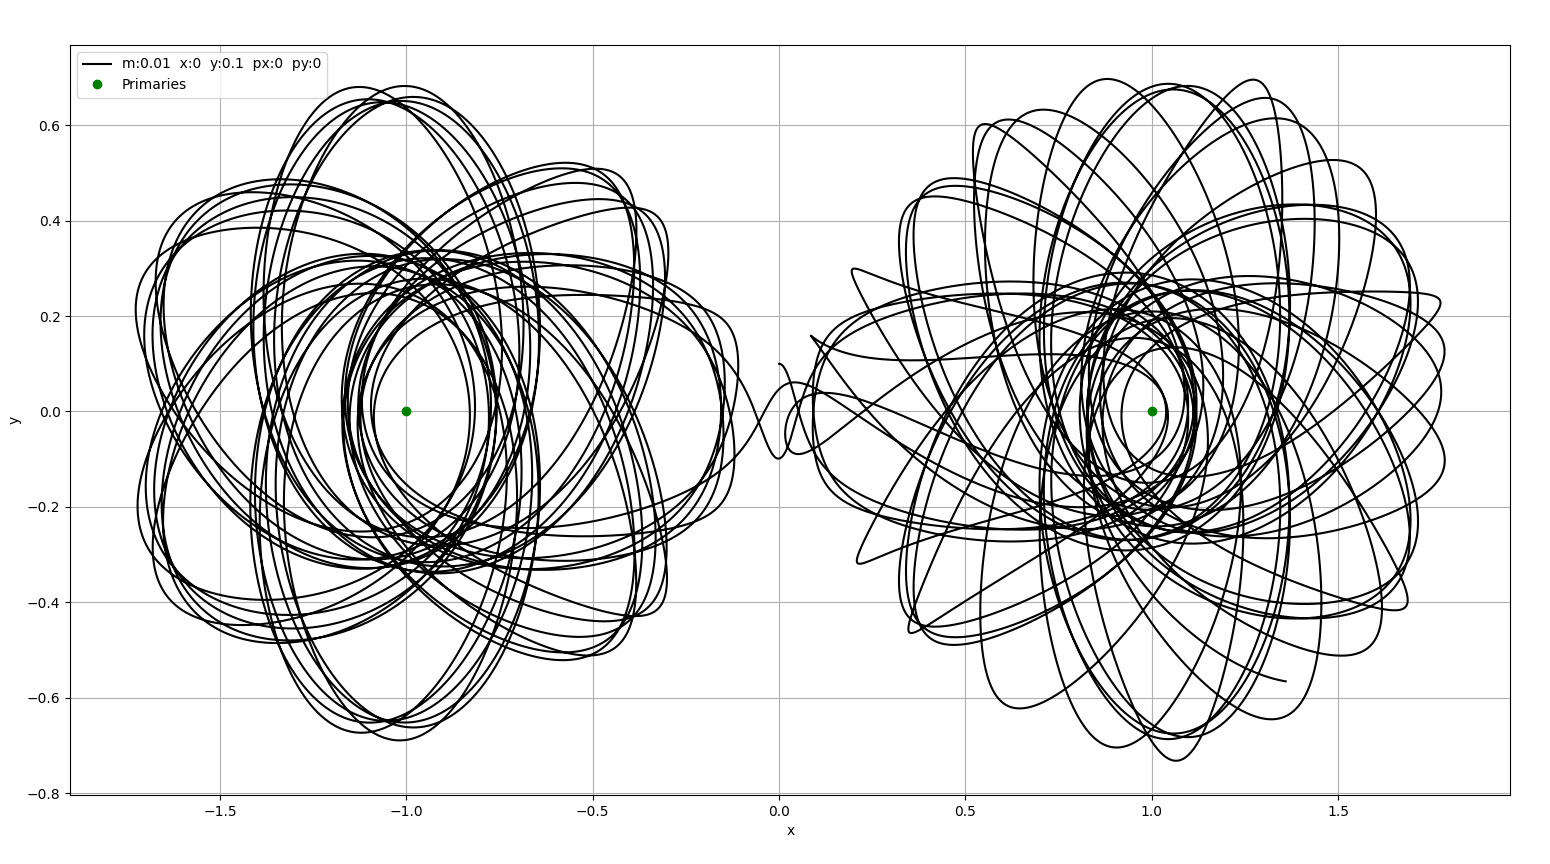
\includegraphics[scale=0.3]{ch14-16.png}
    \end{center}
\end{proof}
\end{document}



















